\documentclass{article}
\usepackage[utf8]{inputenc}

\title{Example-Project}
\author{harallon }
\date{December 2016}

\usepackage{natbib}
\usepackage{graphicx}

\begin{document}

\maketitle

\section{Github Update}
This section is to test the synchronise to GitHub. 

\section{Test Project}
This is simply a test project made by Harald Lønsethagen to see how many I can share with simultaneously.
Can i edit this?

\section{Introduction}
There is a theory which states that if ever anyone discovers exactly what the Universe is for and why it is here, it will instantly disappear and be replaced by something even more bizarre and inexplicable.
There is another theory which states that this has already happened.

\begin{figure}[h!]
\centering
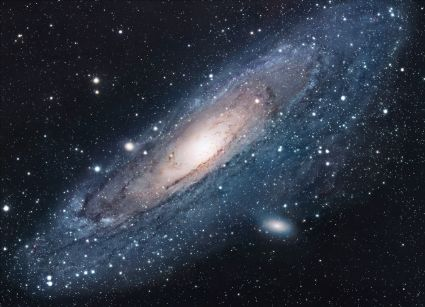
\includegraphics[scale=1.7]{universe.jpg}
\caption{The Universe}
\label{fig:univerise}
\end{figure}

\section{Conclusion}
``I always thought something was fundamentally wrong with the universe'' \citep{adams1995hitchhiker}

\bibliographystyle{plain}
\bibliography{references}
\end{document}
